\begin{figure}[h!]
    \centering
    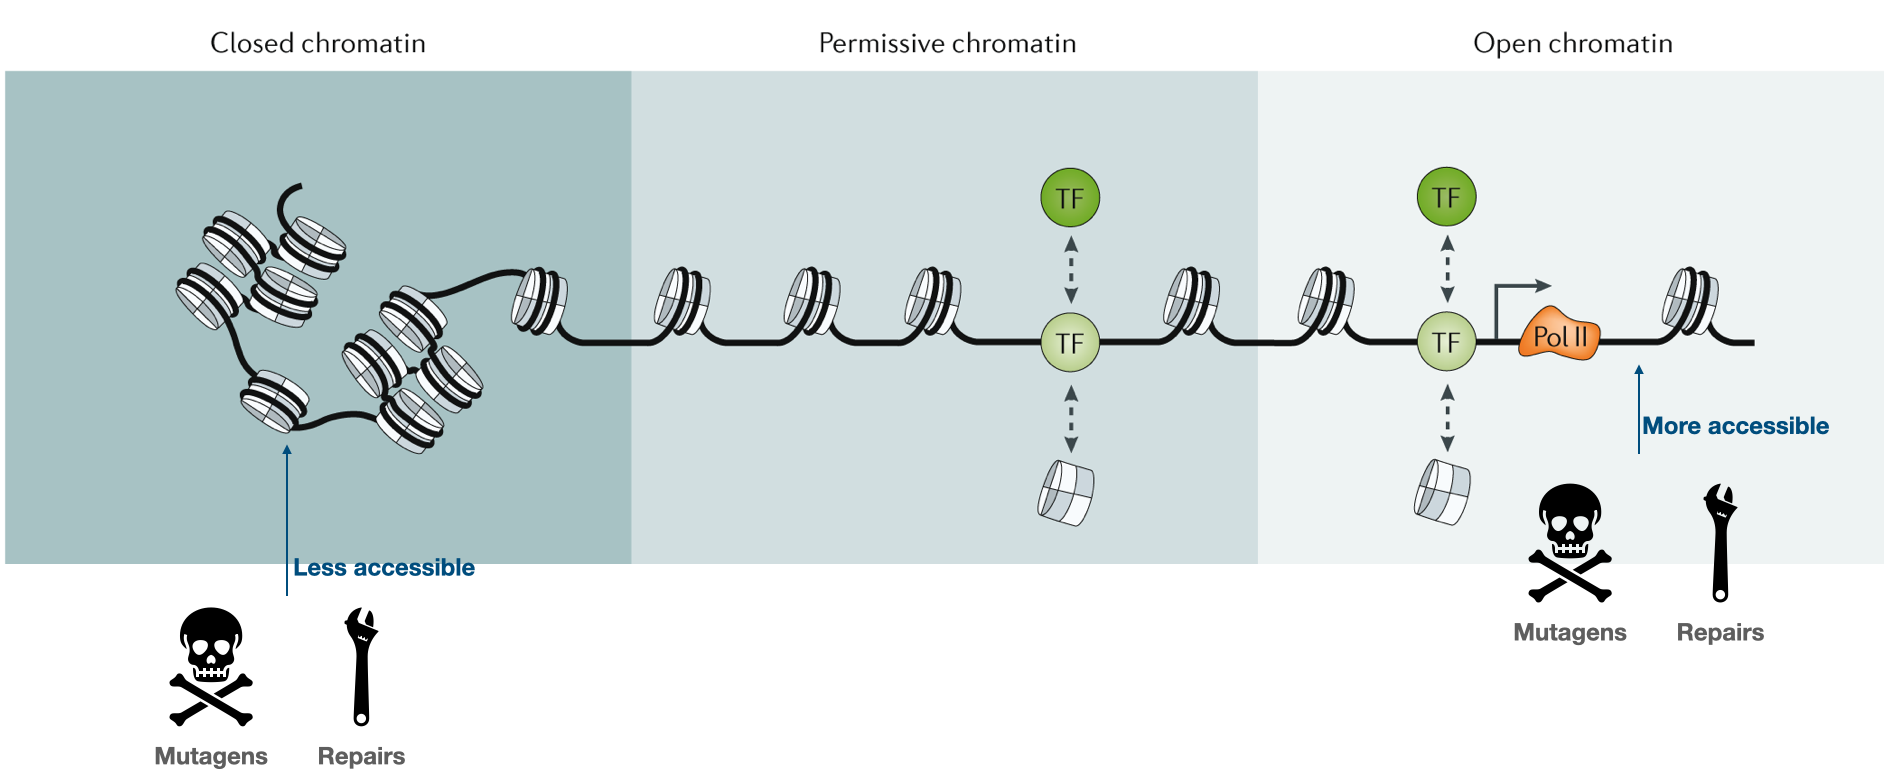
\includegraphics[scale=0.24]{graphics/chromatin_demo.png}
    \caption{\textbf{The distribution of mutations across the genome is hypothetically influenced by cell chromatin structure.} DNA in closed chromatin regions is not accessible to both mutagens and repairs, and is more prone to mutations. Different cell types have different chromatin structures as well as different repair systems, making genomic location effect (GLE) a potential factor that makes a cancer distinct from another. Figure modified from \citet{Klemm2019ChromatinEpigenome}. TF means transcription factor, Pol II means polymerase II}.
    \label{fig:chromatin_demo}
\end{figure}
